\documentclass[]{report}
\usepackage[dvipsnames]{xcolor}
\usepackage{float}
\usepackage{parskip}
\usepackage[top=45mm, bottom=45mm, left=25mm, right=25mm]{geometry}
\usepackage{listings}
\usepackage{tikz}
\usetikzlibrary{shadows,shapes,positioning}
\usepackage{amsmath}
\usepackage{amssymb}
\usetikzlibrary{positioning, shapes.geometric, arrows}
\usepackage{mathrsfs}
\usepackage{booktabs}
\usepackage{enumitem}
\usepackage[hidelinks]{hyperref}


\renewcommand{\arraystretch}{1.5}

\tikzset{
	block/.style n args={1}{
		draw, % Draw a border
		rectangle, % Shape of the node
		minimum height=10 em, % Minimum height of the node
		minimum width=1.5em, % Minimum width of the node
		align=center, % Text alignment within the node
		% Apply fill color based on parameter
		fill=#1
	}
}

\title{Final Project \\ \textasciitilde \\ \textbf{EEG Dataset Classifier}}
\date{\textit{April 8, 2024}}
\author{
	Arnav Goyal - 251244778 \\
	Graeme Watt - 251201502
}
\lstset{
	basicstyle=\ttfamily,
	frame=single,
	language=Python
}


\usepackage[T1]{fontenc}
\usepackage{tgpagella}

\begin{document}
	
\maketitle

\section*{Overview}

In this report, we will talk about our Final Project, where we used a pytorch classifier to predict classes of the dataset in Task 3, more specifically the \href{https://github.com/PerforMance308/EEG_Dataset}{\underline{EEG Brain DE Features Dataset}}. This dataset will be referred to as \textit{the dataset} from here on out. Furthermore our entire codebase can be found at my (arnav’s) \href{https://github.com/arnav57/university/tree/main/Winter%202023-2024/AISE%203010/Final%20Proj}{\underline{github repository}}. I already had a repository for everything in this year, and i was too lazy to add Graeme to the repository, so all the commits are from me (arnav), but we both worked on the code present there equally.

\section*{The Code Base}

Before we start talking about the individual methods and processes present within our codebase, we would like to present a brief overview of our entire codebase and explain the purpose of each file. The files/directories present in our code base are listed below.

\begin{itemize}[]
	\item \texttt{root.py}
	\item \texttt{models.py}
	\item \texttt{dataset.py}
	\item \texttt{load\_data.py}
	\item \texttt{hyperparams.json}
	\item \texttt{data/}
	\item \texttt{checkpoints/}
\end{itemize}

\texttt{root.py} is the backbone of our codebase and holds the methods used to test, train, load from and save checkpoints of various models, it also contains the entry point (main method) of the codebase. It works with two other key scripts \texttt{models.py} and \texttt{dataset.py}. \texttt{models.py} is a script that contains pytorch classes with differing network architectures, at the moment it only contains the finalized network we used, but it was useful in holding many different classes during the training stages of the project. \texttt{dataset.py} is a script that casts the data from the dataset into pytorch DataSet classes that work with pytorch DataLoaders. \texttt{load\_data.py} is a script that comes directly from the github of the dataset and we invoke it within the \texttt{dataset.py} script. These 4 files are the only script files in the entire codebase, the other files are just for storage/modification purposes.

The \texttt{hyperparams.json} file holds the training parameters the script uses for training. Its data can be changed easily to alter the training hyperparameters. The \texttt{data/} directory must be present within the codebase as this is where the dataset is downloaded to. The \texttt{checkpoints/} directory must also be present in the codebase. In the file we provide as a submission, this directory will contain a state dictionary with our most accurate model, which you can easily load by running \texttt{root.py}, this will be explained later in the report.

\newpage

\section*{Method Descriptions}

Now we will describe the methods present within each file in our codebase.

\texttt{root.py}
\begin{itemize}
	\item \texttt{train()}: trains a model according to some architecture which can be defined in this script, using some defined hyperparameters in \texttt{hyperparameters.json}, on the training part of the EEG dataset. It has a nice progress bar and shows the training curve after the training loop is done.
	
	\item \texttt{test()}: tests a model according to some architecture which can be defined in this script, on the testing portion of the EEG dataset. It also has a nice progress bar and prints the testing accuracy after completion of the testing loop
	
	\item \texttt{printInfo()}: displays the class name of the model being trained, the device on which it is being trained on, the optimizer it is using, and the training hyperparameters used, these hyperparameters are located in \texttt{hyperparameters.json}.
	
	\item \texttt{plot()}: assumes the list passed into the function is a list of losses per epoch, it plots them against epoch, and displays them with labeled axes.
	
	\item \texttt{save\_weights()}: prompts the user of the program for input, and either saves weights to the \texttt{checkpoints/} directory as a \texttt{.pth} file or discards them.
	
	\item \texttt{load\_weights()}: prompts the user of the program for input, and either loads the model architecture from a \texttt{.pth} file located in the \texttt{checkpoints/} directory that is compatible with the current model architecture chosen, or it loads the current model architecture with random parameters initially
	
	\item \texttt{main()}: holds the main method of the codebase. It tells the user what model architecture they are using, asks if they would like to use any of the saved weights if they exist for that architecture, and then asks the user if they would like to further train the model, or just test the model. Based on the user’s input the program then trains, displays the training curve, tests and prints test accuracy, or it tests and prints test accuracy.	
\end{itemize}

\texttt{dataset.py}
\begin{itemize}
	\item \texttt{eegpca()}: performs principal component analysis (with components that make up 99\% of the variance in the original data) on the training and testing EEG dataset classes.
	
	\item This file also contains the classes \texttt{EEGTrainingData} and \texttt{EEGTestingData} which were created in order to cast the EEG dataset from github to pytorch DataSet classes so that we can use them in pytorch DataLoaders
\end{itemize}

\texttt{load\_data.py}
\begin{itemize}
	\item \texttt{maybe\_download()}: If there is no directory of the predefined DATA\_DIRECTORY name, the function makes a directory with that name. If there is no file within DATA\_DIRECTORY, the function downloads the dataset file from the SOURCE\_URL.
	
	\item \texttt{dense\_to\_one\_hot()}: Takes the labeled class data, and using one-hot encoding, translates it to have three features per datapoint, one for each of the three classes being predicted.
	
	\item \texttt{load\_data()}: opens the passed filename, and using pickle, encodes the file data into a dictionary. After splitting the dictionary into data and labels, uses \texttt{dense\_to\_one\_hot()} if it is not already one-hot encoded, and returns the data and labels
	
	\item \texttt{DataSet()}: a class containing an \texttt{\_\_init\_\_()} function, 4 property functions, and one other function, this was not used in our code. However we are still going to document it.
	\begin{itemize}[]
		\item \texttt{\_\_init\_\_():} Asserts the length of the data and labels being passed are equal. Sets the \_num\_examples variable as the length of the data, \_data as the passed data, \_labels as the passed labels, \_epochs\_completed, and \_index\_in\_epoch equal to zero.
		
		\item \texttt{@property data()}: Returns the object’s \_data variable
		
		\item \texttt{@property labels()}: Returns the object’s \_labels variable
		
		\item \texttt{@property num\_examples(}): Returns the object’s \_num\_examples variable
		
		\item \texttt{@property epochs\_completed()}: Returns the object’s \_epochs\_completed variable
		
		\item \texttt{next\_batch()}: Increases the \_index\_in\_epoch by the passed batch\_size variable. If \_index\_in\_epoch is greater than \_num\_examples, \_epochs\_completed is incremented by 1, the data and corresponding labels are randomly shuffled, \_index\_in\_epoch is set to the batch\_size, and batch\_size is asserted to be less than or equal to \_num\_examples. Finally, a slice of \_data and \_labels are returned, from the start position (\_index\_in\_epoch at the start of the function call), to the end position (\_index\_in\_epoch at the end of the function) \\
	\end{itemize}
	
	\item \texttt{read\_data\_sets()}: Makes a DataSets object, taking an object type, and not specifying a constructor. Makes a train\_filename and test\_filename by calling maybe\_download with “train” and “test” respectively. One-hot encodes the data and labels by calling load\_data with both filenames. Creates a DataSets object, data\_sets, then adding a train and test to data\_sets, with data and labels from the previous step, before returning data\_sets.
	
\end{itemize}

\section*{Dataset Extraction}

Since we are using the EEG dataset, we implemented the methods defined in the GitHub repository. In addition to performing the standard loading that was predefined. This included using the load\_data.py file provided. Within this file, are five library imports, three standalone methods, one class with 6 built in methods, and one method which implements the class

We also performed Principal Component Analysis on the data, to reduce the input featureset from 310 features. After performing three tests of PCA, we found that 16 features were needed to explain 90\% of the variance in the training data, 26 features were needed to explain 95\% of the variance, and 66 features were needed to explain 99\% of the variance. Since even having 66 features was a drastic reduction, nearly five times, compared to the original features, we decided on the 66 feature reduced set, as it would hopefully still give us a high accuracy.

To implement this PCA, all that was needed was a short method called eegpca, in the dataset.py file, and calling eegpca on the trainset and testset within root.py, before making the dataloaders. The code required for eegpca, along with the required import statement has been placed below. 

\textit{Note:} This is the only code snippet in this report, the source code is provided with the submission, which means it would be redundant to place it here as well.

\begin{center}
	\vspace{1em}
\begin{lstlisting}
from sklearn.decomposition import PCA


def eegpca(trainset:EEGTrainingData, testset:EEGTestingData):
pca = PCA(n_components=0.9)
pca.fit(trainset.eeg_train_data)
test_data = pca.transform(testset.eeg_test_data)
testset.eeg_test_data = torch.from_numpy(test_data).float()
train_data = pca.transform(trainset.eeg_train_data)
trainset.eeg_train_data = torch.from_numpy(train_data).float()
\end{lstlisting}
\textbf{Code Snippet 1:} Code required to perform PCA on the EEG dataset
\end{center}

\newpage

\section*{Network Architecture}

The network architecture we used is defined in the models.py file. The most accurate network architecture we were able to find was a network of 6 fully connected layers, with a normalization layer between each pair of layers. For our activation function, we used the ReLu function on the first through fifth layer, and softmax on the final layer, since this is a classification problem. We also chose Cross Entropy Loss as our loss function, Stochastic Gradient Descent with Momentum, SGDM, as our optimizer.

For the individual layers, we began with a fully connected layer with 66 input features, which is the feature size of our reduced dataset, and 128 output features. For each of the subsequent layers, we used “Lazy Linear” layers, which automatically infer the number of input features from the previous layer. This made the rest of the layers have the following number of input and output features:
\begin{itemize}
	\item 66 input, 128 output
	\item 128 input, 256 output
	\item 256 input, 512 output
	\item 512 input, 1024 output
	\item 1024 input, 128 output
	\item 128 input, 3 output
\end{itemize}
The final layer, with 3 output features represents the three classes to predict. This architecture is depicted via a really nicely drawn \LaTeX diagram below.

\begin{center}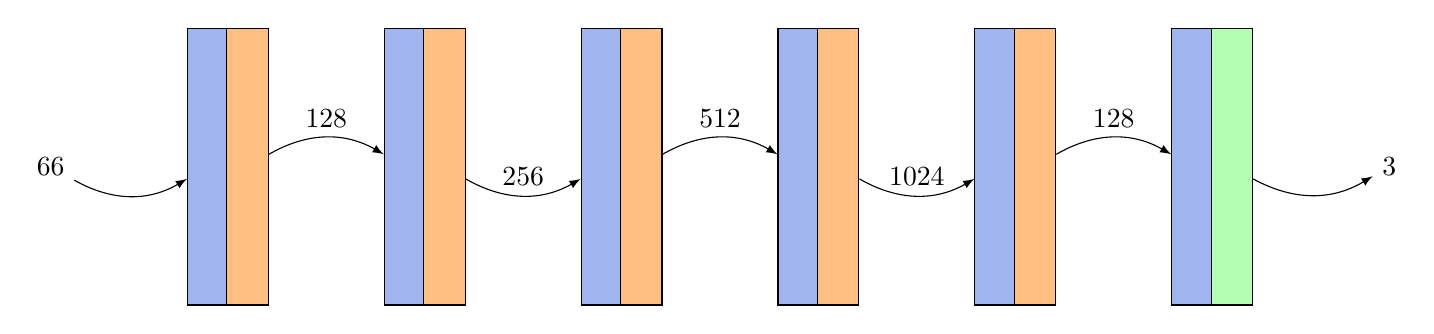
\begin{tikzpicture}[node distance = 0.5cm]
	
	\node[] (orig) {66};
	
	\node[block=RoyalBlue!50, node distance=2cm, right of = orig] (in) {};
	\node[block=orange!50, right of = in] (a0) {};
	\draw[-latex] (orig) to[bend right] node[above, midway] {} (in);
	
	\node[block=RoyalBlue!50, node distance=2cm, right of = a0] (h1) {};
	\node[block=orange!50, right of = h1] (a1) {};
	\draw[-latex] (a0) to[bend left] node[above, midway] {128} (h1);
	
	\node[block=RoyalBlue!50, node distance=2cm, right of = a1] (h2) {};
	\node[block=orange!50, right of = h2] (a2) {};
	\draw[-latex] (a1) to[bend right] node[above, midway] {256} (h2);
	
	\node[block=RoyalBlue!50, node distance=2cm, right of = a2] (h3) {};
	\node[block=orange!50, right of = h3] (a3) {};
	\draw[-latex] (a2) to[bend left] node[above, midway] {512} (h3);
	
	\node[block=RoyalBlue!50, node distance=2cm, right of = a3] (h4) {};
	\node[block=orange!50, right of = h4] (a4) {};
	\draw[-latex] (a3) to[bend right] node[above, midway] {1024} (h4);
	
	\node[block=RoyalBlue!50, node distance=2cm, right of = a4] (h5) {};
	\node[block=green!30, right of = h5] (a5) {};
	\draw[-latex] (a4) to[bend left] node[above, midway] {128} (h5);
	
	\node[right of = a5, node distance=2cm] (out) {3};
	\draw[-latex] (a5) to[bend right] (out);
	
\end{tikzpicture}
\vspace{1em} \\
\textbf{Architecture 1:} The architecture we used for the classifier. \\
\textit{The {\color{RoyalBlue} blue blocks} represent linear pytorch layers, the {\color{orange} orange blocks} represent the relu activation, the {\color{green} green block} represents a concluding softmax activation. The number of features through the model is shown on the arrows. }
\end{center}

\newpage

\section*{Results \& Verification}

After training our model with a batch size of 32, for 20 epochs at a learning rate of 0.001 and momentum of 0.85 we produced a model that can obtain a testing accuracy of 79.46\%, We were supposed to average it over two test runs, but our model attains this accuracy every time during the testing loop.

\begin{center}
	
	\includegraphics[scale=0.45]{verified_ss} \\ 
	\vspace{1em}
	\textbf{Image 1:} The verified 79.46\% accuracy on our VSCode environment
	
\end{center}

In order to verify this result yourself, extract our entire submission into a folder and run root.py to download the dataset, once the dataset is downloaded you should see a prompt asking you if you would like to load a train checkpoint. Enter a 1 into the console to load our pretrained model located at checkpoints/NeuralNet.pth. After that the program will ask if you want to train further, or test the model. In this scenario enter a 2 into the console and the program will begin the testing loop, and will print testing accuracy after it is completed. If you have any questions related to program execution please email: agoyal57@uwo.ca and gwatt23@uwo.ca 

\end{document}
